%Geamtübersicht Messgebiet
\section{Das Hegau}

Das Hegau ist ein Gebiet, das grob zwischen dem Bodensee und der schwäbischen Alb liegt(Wikipedia)???. Charakteristisch für dieses Gebiet sind die vulkanisch 
geprägten Hegauer Kegelberge. Diese Kegelberge sind Schlote erloschener Vulkane. Der Vulkanismus des Hegaugebiets hat seinen Ursprung in der Mitte des Miozän, 
was vor etwa 14 Millionen Jahren war. Es entstanden dutzende Vulkane, in deren Schloten vor ca. 9 Millionen Jahren auch der Hegauer Basalt erstarrte.
Im Pleistozän gab es eine Eiszeit in diesem Gebiet. Durch die entstandenen Gletscher wurde Molasse und Tuff abgetragen, es blieben, die heute noch zu sehenden, 
Phonolithkerne und Basaltkerne stehen. 

\section{Die Messgebiete}
\label{sec:Messgebiete}

Während der Messwoche zelteten wir auf einem Campingplatz in Engen. Von dort aus fuhren wir jeden Tag zu unserem Messgebiet A59/1, das in Abbildung \ref{abb:Messgebietegro} auf der Karte zu sehen ist.

\begin{figure}[ht]
 \centering
 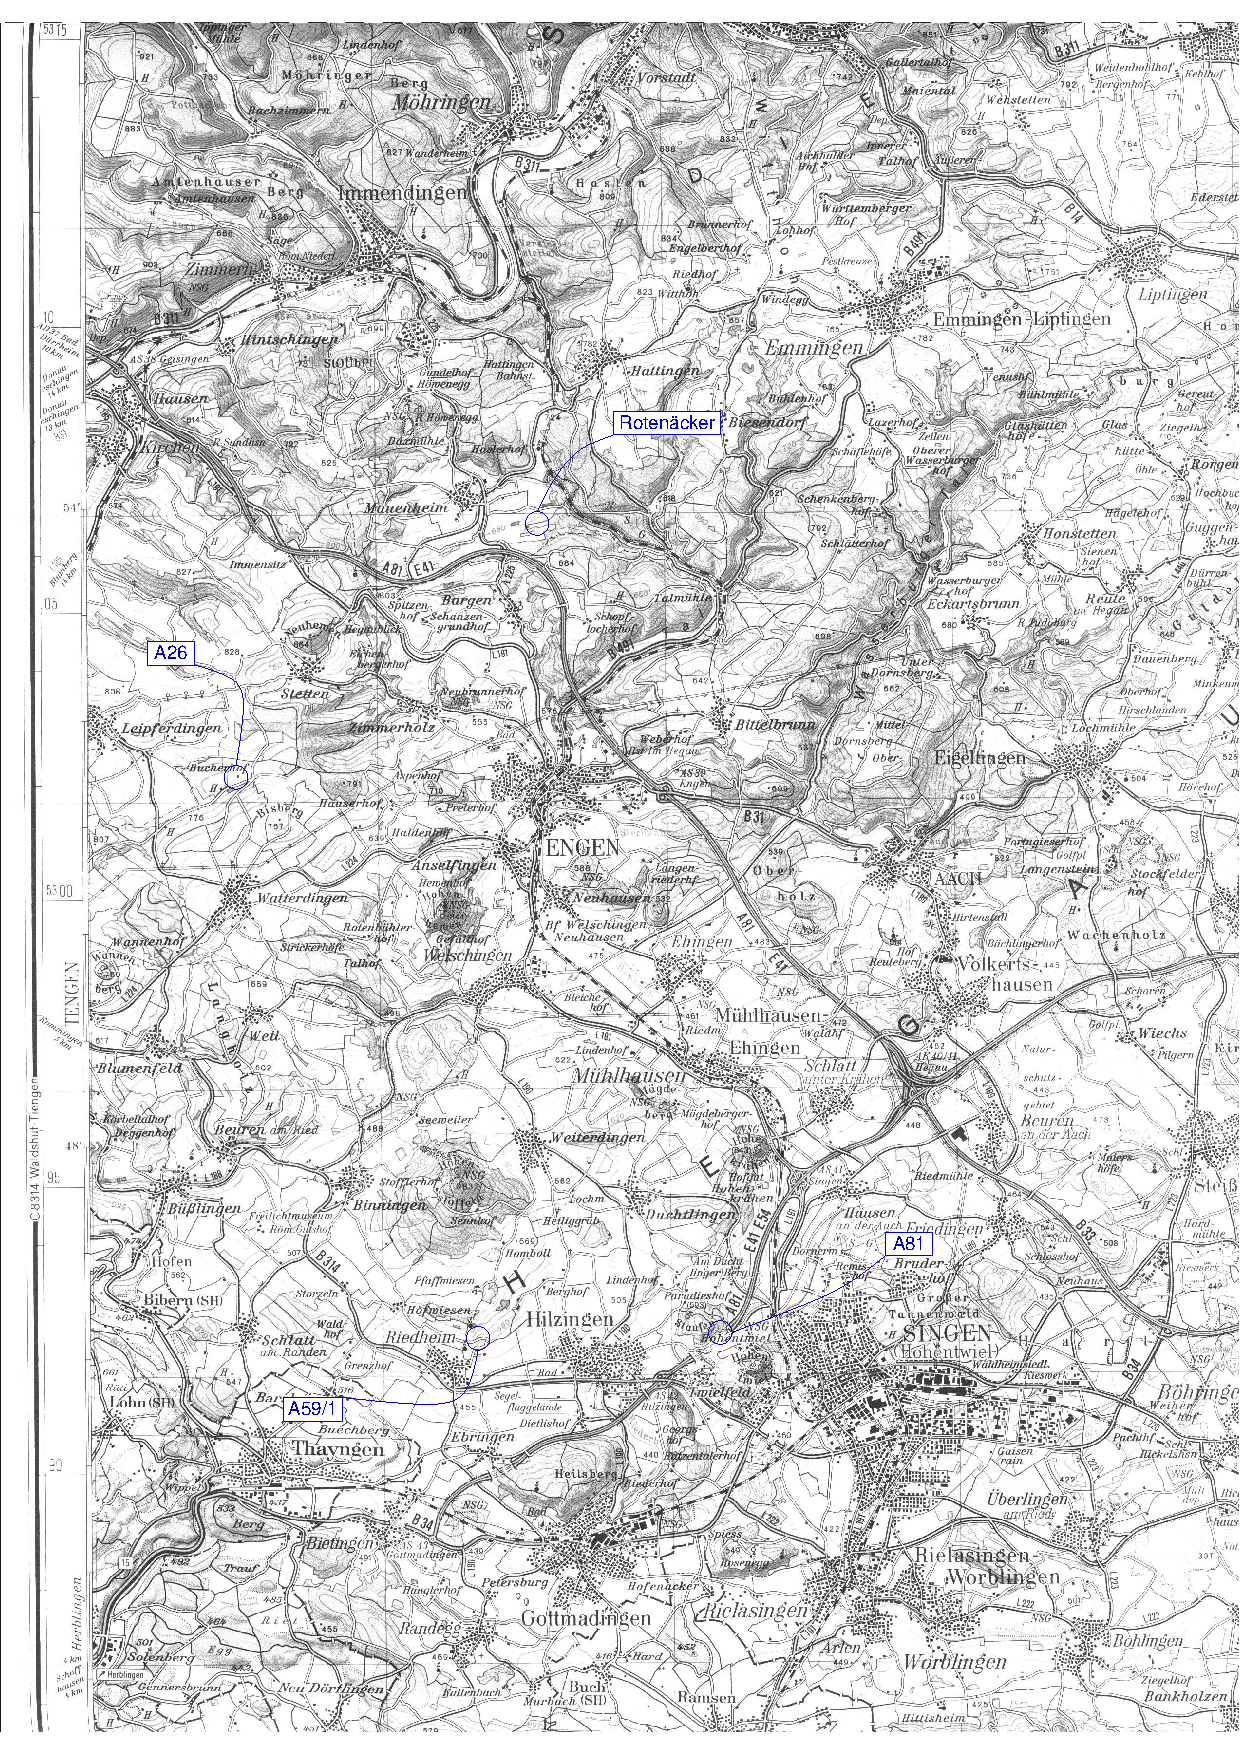
\includegraphics[width=0.75\textwidth]{fig/Uebersichtskarte.pdf}
 \caption[Messstandorte]{Messstandorte, auf denen die Geländeübung durchgeführt wurde. Unser Messstandort Riedheim ist unten links (A59/1) eingezeichnet.}
 \label{abb:Messgebietegro}
\end{figure}

Es gab im Wesentlichen zwei Messgebiete auf denen wir unsere Messungen durchgeführt haben. Sie liegen über Riedheim. In Abbildung \ref{abb:Messgebiete} sind diese Messgebiete 
eingezeichnet. Unter Messgebiet 1 liegt der Basaltgang. Hier wurden mit allen vier Messmethoden Messungen durchgeführt. 
Auf Messgebiet 2 wurde nur mit der Geoelektrik und Seismik gemessen.

\begin{figure}[ht]
 \centering
 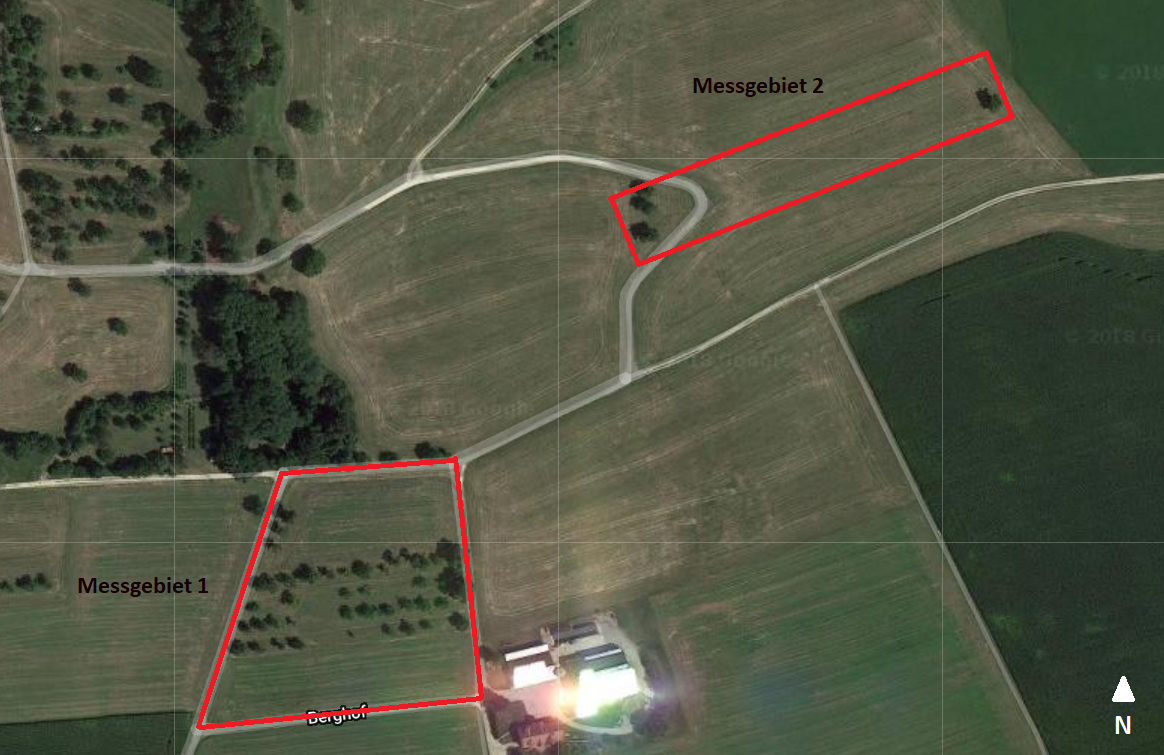
\includegraphics[width=0.9\textwidth]{fig/Messgebiete.png}
 \caption[Messgebiete]{Messgebiete, auf denen unsere Messungen durchgeführt wurden. Unter Messgebiet 1 ist der Basaltgang. Die Graphik wurde von Rebekka Kirchgässner und Luisa Rank übernommen.}
 \label{abb:Messgebiete}
\end{figure}

Oberhalb den Messgebiets 1 ist ein Steinbruch, in dem Basalt freigelegt ist. Der Aufschluss dieses Basaltgangs ist etwa 5 Meter hoch und 16 Meter breit. 
Es ist zu erkennen, dass der Basalt nicht im ganzen Aufschluss in gleichem Zustand vorliegt. In der Mitte sieht er wesentlich kompakter aus als an den Rändern.
Dieser Basaltgang geht unterirdisch weiter und läuft schräg durch das Messgebiet 1. Bei den meisten unserer Messungen wurde dieser Basaltgang untersucht.

In Abbildung \ref{abb:Geolog} ist eine geologische Karte unseres Messgebiets zu sehen. In der Mitte ist in schwarz der Basaltgang oberhalb des Steinbruchs zu sehen, denn dort wurde er sicher nachgewiesen.
Unterhalb des Steinbruchs ist die Lage des Basaltgangs durch zwei gestrichelte Linien angegeben, da hier nicht eindeutig nachgewiesen wurde, ob es sich bei dieser magnetischen Anomalie um Basalt handelt. Der Untergrund unter dem Messgebiet 1 besteht nach dieser Karte aus älterem Juranagelfluh. Dies wurde der Legende der Karte entnommen. Das Messgebiet 2 liegt teilweise über älterem Juranagelfluh und oberer Süßwassermolasse.

\begin{figure}[ht]
 \centering
 \includegraphics[width=\textwidth]{fig/Geolog.pdf}
 \caption[Geologische Karte]{Geologische Karte des Messstandorts Riedheim}
 \label{abb:Geolog}
\end{figure}